\chapter{Datenanalyse und Trainingsvorbereitung} 
\label{chap:datenanalyse_und_trainingsvorbereitung} 

\section{Ausgangsdaten} 

\subsection{Artikeldaten}
\label{sec:artikeldaten} 

Die Artikeldaten liegen in XML-Dateien vor. 
XML (\textit{Extensible Markup Language}) ist ein standardisiertes Format zur strukturierten Speicherung technischer Informationen. 
Durch die hierarchische Struktur können sowohl einfache Stammdaten als auch komplexe technische Eigenschaften abgebildet werden. 
Die Analyse der Artikeldaten hat ergeben, dass sie eine Vielzahl technischer Eigenschaften enthalten, darunter: 

\begin{itemize} 
    \item Herstellerinformationen, 
    \item Typ- und Bestellnummern, 
    \item Spannungen, 
    \item Ströme, 
    \item Leistungen,  
    \item Kommunikationsschnittstellen, 
    \item technische Hinweise, 
    \item Referenzen auf zugehörige Makros. 
\end{itemize} 

Um diese Eigenschaften anhand des Motorbeispiels aus Kapitel \ref{sec:herleitung} zu veranschaulichen, soll hierfür ein Motor von SEW betrachtet werden.
Abbildung \ref{fig:xml_artikel_motor} zeigt die beispielhafte Struktur eines XML-Artikels für diesen Motor.

\begin{figure}[H] 
    \centering 
    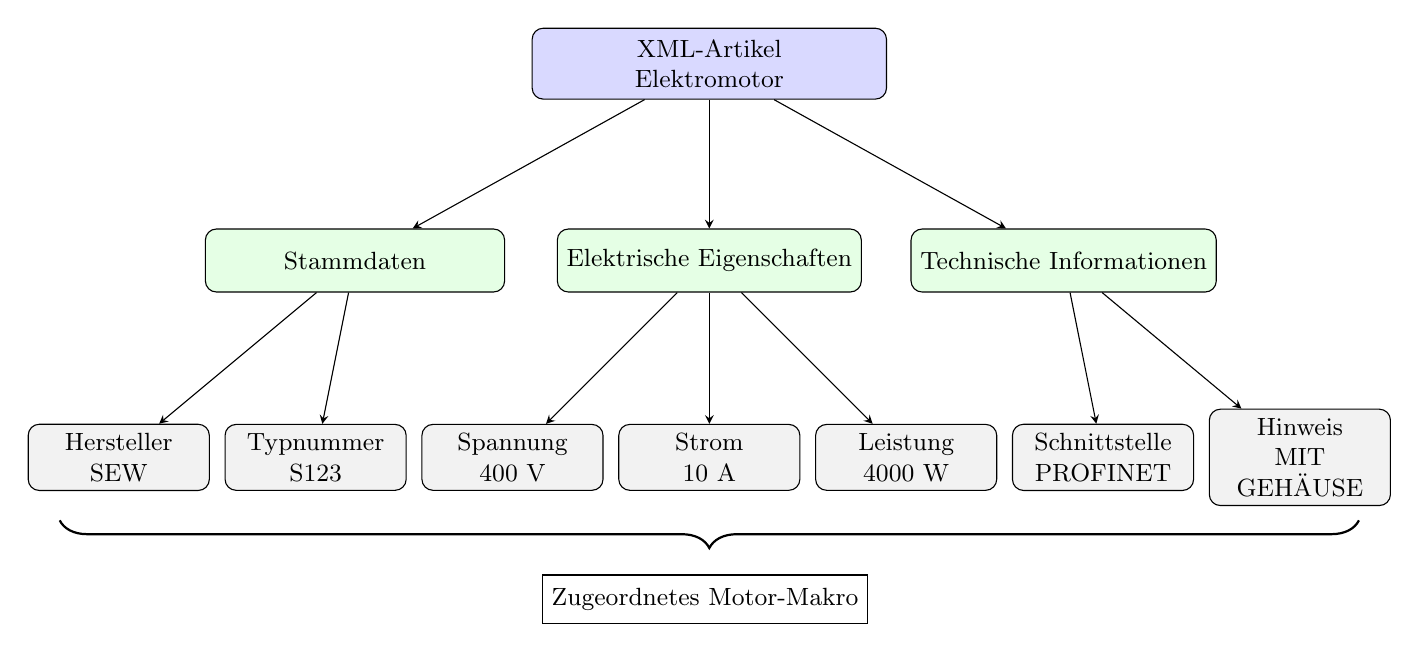
\begin{tikzpicture}[>=stealth, font=\small, 
        every node/.style={align=center}, 
        root/.style={ draw, rounded corners, 
        fill=blue!15, minimum width=4.5cm, minimum height=0.9cm }, 
        category/.style={ draw, rounded corners, fill=green!10, minimum width=3.8cm, minimum height=0.8cm }, 
        feature/.style={ draw, rounded corners, fill=gray!10, minimum width=2.3cm, minimum height=0.8cm, align=center } ] 
        % Wurzel 
        \node[root] (article) at (0,5) {XML-Artikel\\Elektromotor}; 
        % Kategorien 
        \node[category] (master) at (-4.5,2.5) {Stammdaten}; 
        \node[category] (electrical) at (0,2.5) {Elektrische Eigenschaften}; 
        \node[category] (technical) at (4.5,2.5) {Technische Informationen};
        % Verbindungen 
        \draw[->] (article) -- (master); 
        \draw[->] (article) -- (electrical); 
        \draw[->] (article) -- (technical); 
        % Stammdaten 
        \node[feature] (manu) at (-7.5,0) {Hersteller\\SEW}; 
        \node[feature] (type) at (-5.0,0) {Typnummer\\S123}; 
        \draw[->] (master) -- (manu); 
        \draw[->] (master) -- (type);
        % Elektrische Eigenschaften 
        \node[feature] (voltage) at (-2.5,0) {Spannung\\400 V}; 
        \node[feature] (current) at (0,0) {Strom\\10 A}; 
        \node[feature] (power) at (2.5,0) {Leistung\\4000 W};
        \draw[->] (electrical) -- (voltage); 
        \draw[->] (electrical) -- (current); 
        \draw[->] (electrical) -- (power); 
        % Technische Informationen 
        \node[feature] (ip) at (5.0,0) {Schnittstelle\\PROFINET}; 
        \node[feature] (com) at (7.5,0) {Hinweis\\MIT\\GEHÄUSE};
        \draw[->] (technical) -- (ip); 
        \draw[->] (technical) -- (com); 
        % Makro
        \draw[ decorate, decoration={brace,mirror,amplitude=10pt}, thick ] (-8.25,-0.8) -- (8.25,-0.8) node[midway,yshift=-1cm] { \fbox{\strut Zugeordnetes Motor-Makro} };
    \end{tikzpicture} 
    \caption{Beispielhafte Struktur eines XML-Artikels für einen Elektromotor. Die hierarchische Organisation ermöglicht die Speicherung von Herstellerinformationen, elektrischen Eigenschaften, technischen Merkmalen sowie Referenzen auf zugehörige Makros.} 
    \label{fig:xml_artikel_motor}
\end{figure}

\subsection{Makrodaten} 

Neben den Artikeln werden die zugehörigen Makros analysiert. Die Makros werden im .ema-Format gespeichert. 
Dieses Format entspricht einem XML-basierten Schema, das sowohl grafische als auch technische Informationen strukturiert abbildet. 

Hierzu gehören: 

\begin{itemize} 
    \item Anschlussstrukturen,  
    \item Makrovarianten,   
    \item Bezeichnungen. 
\end{itemize} 

Während die Artikeldaten beschreiben, welche technischen Eigenschaften ein Gerät besitzt, 
beschreiben die Makros die technische Umsetzung dieser Eigenschaft innerhalb eines Schaltplans. 
Beide Informationsquellen ergänzen sich daher gegenseitig. 

Die Bezeichnungen eines Makros werden nach folgendem Muster aufgebaut: Makro-Familie-Variante (z.\,B. M1\_F1\_V1)
Dabei gibt Makro die Nummerierung des Makros selbst an, die Familie beschreibt eine Unterkategorie des Makros und die Variante kennzeichnet unterschiedliche Ausführungen innerhalb dieser Familie.
Im Fall des Motorbeispiels aus Kapitel \ref{sec:herleitung} lässt sich die Bezeichnung M1\_F1\_V1 wie folgt interpretieren:

\begin{itemize}
    \item  M1: Motor
    \item  F1: Gleichstrommotor
    \item  V1: Mit Kühlung
\end{itemize}

Die Abbildung \ref{fig:ema_motor_macro} gibt die Struktur eines Motor-Makros im .ema-Format wieder.

\begin{figure}[H] 
    \centering 
    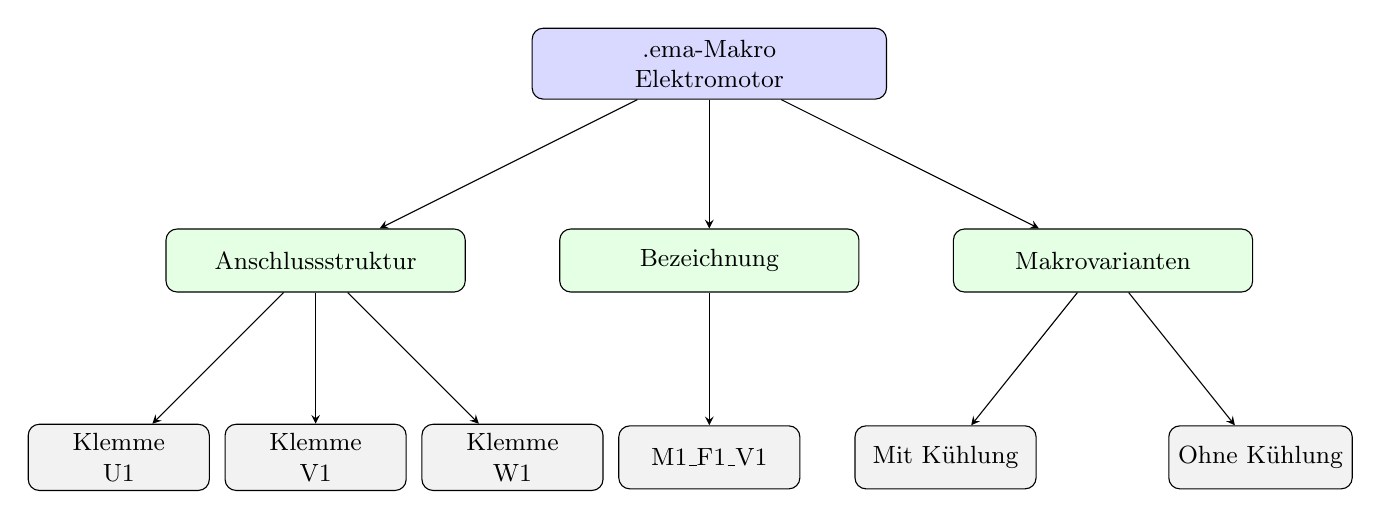
\begin{tikzpicture}[>=stealth, font=\small, 
        every node/.style={align=center}, 
        root/.style={ draw, rounded corners, 
        fill=blue!15, minimum width=4.5cm, minimum height=0.9cm }, 
        category/.style={ draw, rounded corners, fill=green!10, minimum width=3.8cm, minimum height=0.8cm }, 
        feature/.style={ draw, rounded corners, fill=gray!10, minimum width=2.3cm, minimum height=0.8cm, align=center } ] 
        % Wurzel 
        \node[root] (macro) at (0,5) {.ema-Makro\\Elektromotor}; 
        % Kategorien 
        \node[category] (terminal) at (-5.0,2.5) {Anschlussstruktur}; 
        \node[category] (function) at (0,2.5) {Bezeichnung}; 
        \node[category] (variant) at (5.0,2.5) {Makrovarianten}; 
        % Verbindungen 
        \draw[->] (macro) -- (terminal); 
        \draw[->] (macro) -- (function); 
        \draw[->] (macro) -- (variant); 
        % Anschlussstruktur 
        \node[feature] (u1) at (-7.5,0) {Klemme\\U1}; 
        \node[feature] (v1) at (-5.0,0) {Klemme\\V1}; 
        \node[feature] (w1) at (-2.5,0) {Klemme\\W1}; 
        \draw[->] (terminal) -- (u1); 
        \draw[->] (terminal) -- (v1); 
        \draw[->] (terminal) -- (w1); 
        % Bezeichnung 
        \node[feature] (motor) at (0,0) {M1\_F1\_V1}; 
        \draw[->] (function) -- (motor); 
        % Varianten 
        \node[feature] (left) at (3.0,0) {Mit Kühlung}; 
        \node[feature] (right) at (7.0,0) {Ohne Kühlung}; 
        \draw[->] (variant) -- (left); 
        \draw[->] (variant) -- (right); 
    \end{tikzpicture} 
    \caption{Beispielhafte Struktur eines Motor-Makros im .ema-Format. Das Makro beschreibt die technische Umsetzung eines Elektromotors im Schaltplan und enthält Informationen zu Anschlussstrukturen, Bezeichnungen und Makrovarianten.} 
    \label{fig:ema_motor_macro} 
\end{figure}

\subsection{Artikel-Makro-Zuordnungen} 

Die Zuordnung von Artikel zu Makro erfolgt durch die Referenzierung des Makros über die Artikel-Eigenschaft \texttt{P\_ARTICLE\_MACRO}.
Diese Zuordnung kann als n zu 1 Beziehung betrachtet werden, da mehrere Artikel auf dasselbe Makro verweisen können.

Bildlich kann dies wie folgt dargestellt werden: 

\begin{figure}[htbp] 
    \centering 
    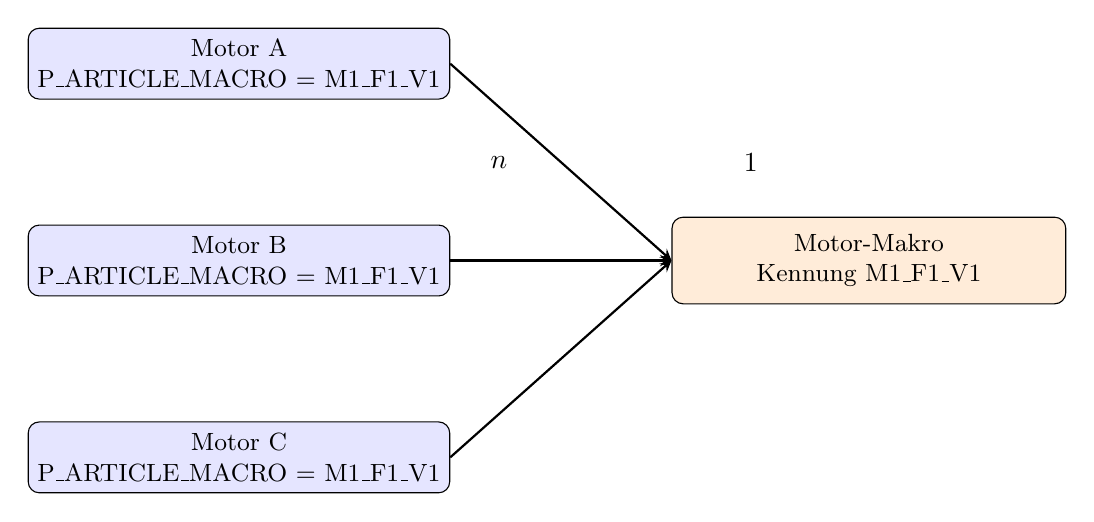
\begin{tikzpicture}[ >=stealth, font=\small, 
        article/.style={ draw, rounded corners, fill=blue!10, minimum width=4cm, minimum height=0.9cm, align=center }, 
        macro/.style={ draw, rounded corners, fill=orange!15, minimum width=5cm, minimum height=1.1cm, align=center } ] 
        % Artikel 
        \node[article] (a1) at (0, 2.5) {Motor A\\P\_ARTICLE\_MACRO = M1\_F1\_V1}; 
        \node[article] (a2) at (0, 0) {Motor B\\P\_ARTICLE\_MACRO = M1\_F1\_V1}; 
        \node[article] (a3) at (0,-2.5) {Motor C\\P\_ARTICLE\_MACRO = M1\_F1\_V1}; 
        % Makro 
        \node[macro] (m1) at (8,0) {Motor-Makro\\Kennung M1\_F1\_V1}; 
        % Verbindungen 
        \draw[->,thick] (a1.east) -- (m1.west); 
        \draw[->,thick] (a2.east) -- (m1.west); 
        \draw[->,thick] (a3.east) -- (m1.west); 
        % Kardinalitäten 
        \node[font=\bfseries] at (3.3,1.25) {$n$}; 
        \node[font=\bfseries] at (6.5,1.25) {$1$}; 
    \end{tikzpicture} 
    \caption{Beispiel einer n:1-Beziehung zwischen Artikeln und Makros. Mehrere Artikel verweisen über die Eigenschaft \texttt{P\_ARTICLE\_MACRO} auf dasselbe Makro.} 
    \label{fig:artikel_macro_n_zu_1} 
\end{figure}

\section{Datenaufbereitung} 

Die eigentliche Datenaufbereitung erfolgt innerhalb der Pipeline-Schritte 911 und 913. 
Ziel dieser Schritte ist die Überführung der heterogenen Rohdaten in einen konsistenten Trainingsdatensatz. 

\subsection{Architektur der Datenaufbereitung} 

Die Architektur der Datenaufbereitung ist in Abbildung XX dargestellt. 
Die XML-Artikeldaten und die EMA-Makrodaten bilden die beiden Eingabeschnittstellen der Pipeline. 

Im Schritt \texttt{911 Prepare Raw Data} erfolgt die technische Analyse dieser Datenquellen. 
Hierbei werden Merkmale extrahiert, normiert und in strukturierte Vektoren überführt. 
Die resultierenden Daten werden anschließend im Schritt \texttt{913 Filter Training Data} hinsichtlich ihrer Qualität überprüft, 
gefiltert und mit Qualitätsinformationen angereichert. Danach erfolgt im Schritt \texttt{921 Build Datasplit} die Aufteilung in Trainings-, Validierungs- und Testdaten.
Das Ergebnis dieser Verarbeitung bildet Artefakt A1. 

\subsection{Datenqualität} 

Da die Daten aus realen Engineering-Projekten stammen, weisen sie unterschiedliche Qualitätsmerkmale auf. 

Typische Probleme sind: 

\begin{itemize} 
    \item fehlende Werte, 
    \item unterschiedliche Schreibweisen, 
    \item verschiedene Einheiten, 
    \item redundante Datensätze, 
    \item mehrsprachige Beschreibungen, 
    \item Varianten desselben Artikels. 
\end{itemize} 

Zusätzlich enthalten die Rohdaten Informationen wie Bearbeiter, Zeitstempel, Projektnamen oder Dateipfade. 
Diese Informationen besitzen keinen technischen Zusammenhang zur späteren Makrowahl und dürfen deshalb nicht als Trainingssignal verwendet werden. 

\subsection{Einheitennormalisierung} 

Technische Informationen können in unterschiedlichen Einheiten oder Schreibweisen vorliegen. 

Beispielsweise können Spannungen als 

\begin{itemize} 
    \item 24 V, 
    \item 24VDC, 
    \item 0,024 kV 
\end{itemize} 

gespeichert sein. Obwohl alle Angaben dieselbe technische Bedeutung besitzen, würden sie ohne Vorverarbeitung als unterschiedliche Merkmale interpretiert werden. 
Aus diesem Grund werden physikalische Größen auf gemeinsame Basiseinheiten normiert. Zusätzlich werden technische Klassen und Wertebereiche erzeugt. 
Beispielsweise entstehen Spannungsklassen wie: 

\begin{itemize} 
    \item Low Voltage, 
    \item Medium Voltage, 
    \item High Voltage. 
\end{itemize} 

Dadurch können technisch ähnliche Geräte auch dann als ähnlich erkannt werden, wenn ihre numerischen Werte leicht voneinander abweichen. 

\subsection{Qualitätsfilterung} 

Nach der Extraktion erfolgt die Qualitätsprüfung. Hierbei werden Datensätze identifiziert, welche: 

\begin{itemize} 
    \item keine gültige Artikelnummer besitzen, 
    \item keine Zielmakros besitzen, 
    \item keine technischen Merkmale enthalten, 
    \item Leakage-Merkmale enthalten, 
    \item widersprüchliche Fingerprints aufweisen. 
\end{itemize} 

Zusätzlich werden problematische Datensätze in Quarantäne verschoben und nicht für das Training verwendet. 

\section{Trainingsdatenmodell} Maschinelle Lernverfahren können technische Informationen nicht direkt aus XML-Dateien verarbeiten. 
Daher werden die verfügbaren Informationen in numerische Merkmalsräume überführt. Die Pipeline erzeugt hierfür drei spezialisierte Vektormodelle. 

\subsection{Artikelvektor} 

Der Artikelvektor beschreibt die technischen Eigenschaften eines Geräts. Hierzu gehören insbesondere: 
\begin{itemize} 
    \item Hersteller, 
    \item Produktfamilie, 
    \item Produkttyp, 
    \item Spannungen, 
    \item Ströme, 
    \item Leistungen, 
    \item Frequenzen, 
    \item Kommunikationsstandards, 
    \item IP-Schutzklassen, 
    \item Kanalzahlen, 
    \item Anschlussprofile. 
\end{itemize} 
Der Artikelvektor bildet die spätere Suchanfrage des Empfehlungssystems ab. 

\subsection{Makrostrukturvektor} 
Der Makrostrukturvektor beschreibt die technische Struktur eines Makros. Hierzu werden unter anderem Merkmale aus den Function Templates extrahiert: 
\begin{itemize} 
    \item Funktionskategorien, 
    \item Funktionsgruppen, 
    \item Anschlussrollen, 
    \item IO-Schemata, 
    \item Kanalstrukturen, 
    \item Signalanzahlen, 
    \item Varianten, 
    \item Symbolbibliotheken, 
    \item Makrokategorien. 
\end{itemize} 
Function Templates besitzen hierbei eine besondere Bedeutung, da sie die tatsächliche elektrische Struktur eines Gerätes innerhalb eines Schaltplans beschreiben. 

\subsection{Lexikalvektor} 
Nicht alle technischen Informationen liegen in strukturierter Form vor. Viele Informationen befinden sich ausschließlich innerhalb von: 
\begin{itemize} 
    \item Typbezeichnungen, 
    \item Produktserien, 
    \item Kommunikationskennungen, 
    \item technischen Beschreibungen. 
\end{itemize} 
Der Lexikalvektor extrahiert gezielt diese technischen Begriffe. Dabei werden keine vollständigen Artikelnummern oder ERP-Kennungen verwendet, um ein Auswendiglernen einzelner Artikel zu verhindern. 

\subsection{Warum drei getrennte Vektoren?} 

Die Aufteilung in Artikelvektor, Makrostrukturvektor und Lexikalvektor erfolgt bewusst. 
Der Artikelvektor beschreibt die technischen Eigenschaften eines Gerätes. Der Makrostrukturvektor beschreibt die technische Umsetzung innerhalb des Schaltplans. 
Der Lexikalvektor ergänzt beide Informationsquellen um zusätzliche technische Begriffe. 
Durch diese Trennung können die einzelnen Wissensquellen unabhängig voneinander ausgewertet und später gezielt kombiniert werden. 

\section{Datensplit} 

Nach Abschluss der Datenaufbereitung erfolgt die Aufteilung der Daten in Trainings-, Validierungs- und Testdaten. 

\subsection{Verwendete Datengröße} Der aktuelle Datensatz umfasst: 

\begin{itemize} 
    \item 1.559 Artikel, 
    \item 375 Makroziele, 
    \item 2.381 technische Merkmale. 
\end{itemize} 

Diese Zahlen wurden nicht manuell festgelegt. Sie ergeben sich unmittelbar aus den verfügbaren Daten nach Abschluss der Datenbereinigung und Qualitätsfilterung. 

\subsection{Trainings-, Validierungs- und Testdaten} 

Die Pipeline verwendet als Zielkonfiguration zunächst: 
\begin{itemize} 
    \item 60 \% Training, 
    \item 20 \% Validierung, 
    \item 20 \% Test. 
\end{itemize} 

Die reale Verteilung beträgt: 
\begin{itemize} 
    \item 984 Trainingsartikel (63,1 \%), 
    \item 322 Validierungsartikel (20,7 \%), 
    \item 253 Testartikel (16,2 \%). 
\end{itemize} 

Die Abweichung gegenüber der Zielkonfiguration entsteht durch zusätzliche Randbedingungen zur Vermeidung von Leakage. 

\subsection{Leakage-Schutz durch Fingerprints} 

Zur Vermeidung von Data Leakage werden Fingerprints verwendet. Ein Fingerprint beschreibt nicht die Identität eines Artikels, sondern dessen technische Signatur. 
Hierzu werden sämtliche technischen Merkmale eines Artikels zusammengeführt und in eine eindeutige Hashrepräsentation überführt. 
Technisch identische Artikel besitzen dadurch denselben Fingerprint. 
Alle Artikel derselben Fingerprint-Gruppe werden gemeinsam innerhalb desselben Datensplits gehalten. 
Dadurch wird verhindert, dass technisch identische Artikel gleichzeitig in Trainings- und Testdaten erscheinen. Die finale Leakage-Prüfung ergibt: 

\[ Fingerprint\text{-}Konflikte = 0 \] 
Damit existieren keine technisch identischen Datensätze über Split-Grenzen hinweg. 

\subsection{Target-Abdeckung} 

Zusätzlich wird sichergestellt, dass alle Makroziele, welche in Validierungs- oder Testdaten vorkommen, 
bereits im Trainingsbestand vertreten sind. Dadurch wird verhindert, dass die Evaluation durch unbeabsichtigte Cold-Start-Situationen verfälscht wird. 

\section{Kapitelergebnis} 

In diesem Kapitel wurden die verfügbaren Artikel- und Makrodaten analysiert sowie die vollständige Datenaufbereitung beschrieben. 
Die Analyse zeigt, dass die EPLAN-Artikelverwaltung eine umfangreiche technische Wissensbasis bereitstellt. 
Diese Informationen werden innerhalb der Pipeline extrahiert, normiert, qualitätsgesichert und in strukturierte Artikel-, 
Makrostruktur- und Lexikalvektoren überführt. Zusätzlich wurden Mechanismen zur Leakage-Vermeidung und zur validen Aufteilung der Daten implementiert. 

Artefakt A1 besteht damit aus: 
\begin{itemize} 
    \item 1.559 qualitätsgesicherten Artikeldatensätzen, 
    \item 375 Makrozielen, 
    \item den vorhandenen Artikel-Makro-Zuordnungen, 
    \item den erzeugten Artikelvektoren, 
    \item den erzeugten Makrostrukturvektoren, 
    \item den erzeugten Lexikalvektoren, 
    \item einem Merkmalsraum mit 2.381 Features, 
    \item einem leakage-freien Trainings-, Validierungs- und Testsplit. 
\end{itemize} 

Damit liegt erstmals eine vollständige technische Repräsentation der vorhandenen Engineering-Wissensbasis vor. 
Dieses Artefakt beantwortet Forschungsfrage RQ1 und bildet die Grundlage für die Auswahl eines geeigneten Modellansatzes in Kapitel 5.
